\hypertarget{lexique}{%
\chapter{Lexique}\label{lexique}}

\hypertarget{apprentissage-supervisuxe9}{%
\section{Apprentissage supervisé}\label{apprentissage-supervisuxe9}}

C'est une branche de l'IA, visant à créer des programmes capables
d'apprendre, à partir d'exemples labelisés, à classifier au mieux des
objets. Son objectif est d'obtenir un taux d'erreur minimal.

\hypertarget{spike-timing-dependent-plasticity}{%
\section{Spike-timing-dependent
plasticity}\label{spike-timing-dependent-plasticity}}

La (STDP) est une généralisation de l'algorithme de la règle de Hebb,
qui est couramment utilisée dans les SNN pour les expériences
d'apprentissage non supervisées. La plasticité est un processus de
modification du poids des synapses. Cette modification dépend du moment
de déclenchement du potentiel d'action dans les neurones pré et
post-synaptique. Ce processus permet d'expliquer partiellement le
développement cérébral et la mémorisation, en provoquant
potentialisation et dépression à long terme des synapses.

\begin{figure}[!h]
\centering
\includegraphics[width=10cm]{./images/STDP.png}
\caption{STDP}
\end{figure}

La STDP peut être implémentée par des variables locales. En haut : Un
spike présynaptique laisse une trace X\(j\)(\(t\)) qui est lue (flèche)
au moment du spike postsynaptique. Le changement de poids est
proportionnel à cette valeur X\(j\)(\(tn\)) Bas : Un spike
postsynaptique laisse une trace y(\(t\)) qui est lue (flèche) au moment
d'une spike présynaptique.

\hypertarget{winner-take-all}{%
\section{Winner-take-All}\label{winner-take-all}}

\begin{figure}[!h]
\centering
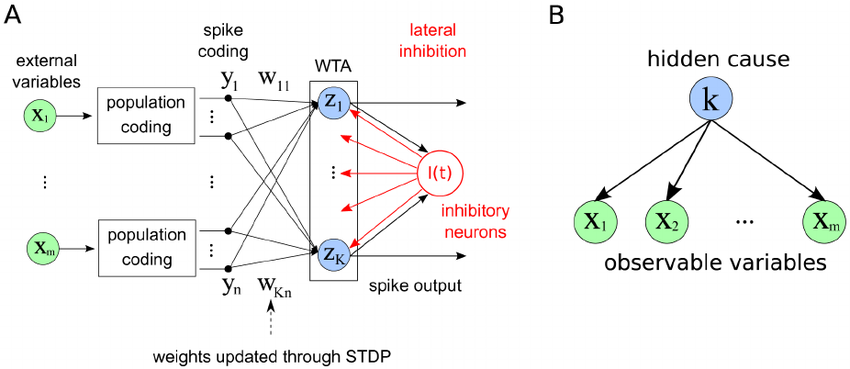
\includegraphics[width=10cm]{./images/image10.png}
\caption{Winner-take-All}
\end{figure}

Le winner-take-all est un principe, ou en gros par rapport a tous ces
spikes que le neurone recevras, cela va faire grimper son potentiel de
membrane, et donc forcement a un moment , il y aura un neurone qui
spike, donc le premier neurone parmi tous les neurones qui spikeras
prendra le dessus sur les autres, pendant que ces autres seront limiter
et ne pourrons spiker en même temps que lui, en gros ce neurone va agir
comme un inhibiteur sur tous les autres. Par exemple ça pourrait
permettre des méthodes d'apprentissage spécialiser par rapport a des
différentes stimulation spécifique pour chaque neurone.
